\section{Methodology}
\label{sec:Meth}

The architecture of our approach can be 
divided into 4 modules, as shown in 
Figure~\ref{fig:netStruct}. 
The first module is image feature extractor, which
contains three pretrained models of DenseNet, which 
are trained on ImageNet task is used as the 
backbone of our network structure. Benefited from 
pre-trained models, the network gains the ability to 
extract basic features from images before training. 
Designing three different models has aimed for 
diverse features. To make use of different 
representation power of each model, fusing the
feature from each model with weight add method.
The second module is a hash decoder, which is aim
at dividing randomly image features into multiple 
branches, with each branch corresponding to one 
hash bit. Through such steps, the model can not 
only improve the generalization ability of the 
model, but also simplify the calculation of 
high-dimensional features to facilitate the work 
of the classifier.
The third module is employed to perform 
classification, we also has 
used three classifiers which contains SVM(Support
Vector Machine), KNN(K Nearest Neighbor) and 
RF(Random Forest). This design of classifications 
is to help improve the accuracy of model 
predictions.
The fourth module is a linear regression analysis 
model, which utilied the RPN(Region Proposal 
Network) proposed by Faster RCNN. To do this, 
it is aimed at marking the specific location of the 
lesion in mammography.

\subsection{Network design}
\label{sec:MethNet}

Hand-crafted features have been widely used in the
image classification tasks, including mammography 
image classification tasks. Though these 
hand-crafted feature based methods perform well, 
they are always too complicated to build and could 
be constrained in specific situations. With the 
development of deep learning techniques, deep 
convolutional neural networks have achieved 
great success in image analysis task, because of 
its ability to extract intricate features from 
raw data
\cite{Szegedy2016,Zeiler2014}.
By training a model with a huge amount of images, 
the learned parameters network could gain greater 
representation power and perform better than 
hand-crafted feature based methods
\cite{Jamieson2012}.
Hence we decide to build a mammography images 
object detection network. CNNs based approaches 
on mammography image 
recognition tasks have been proposed in recent 
years, most of them train a single neural network 
model to extract image features
\cite{He2019}.
After AlexNet achieved great success in the 
ImageNet competition, the potential of deep CNNs 
are gradually discovered by researchers, many deep 
network architectures with good performance on 
image classification tasks such as VGGNet, 
GoogLeNet, ResNet, DenseNet and etc, network 
based on these well-performed architectures are 
naturally applied to mammography image recognition 
task. We build a fusion network made of four 
modules which are feature extractor(Explained 
in detail in 
Section~\ref{sec:MethNetFea}), 
hash decoder(Explained in detail in 
Section~\ref{sec:MethNetHash}),
classifier(Explained in detail in 
Section~\ref{sec:MethNetCls}) 
and regression model(Explained in detail in 
Section~\ref{sec:MethNetReg}). 

\subsubsection{Feature Extract Module}
\label{sec:MethNetFea}

In the feature extractor modules, building it 
with a truncated DenseNet without the fully 
connected layers. The backbone of DenseNet
consists of 3 dense blocks, each dense block 
is composed of several dense layers. The 
number of dense layers in each dense block 
increases while the dense blocks go deeper.
The structure of a dense block is shown in 
Figure~\ref{fig:DenseBlock}.

\begin{figure*}[!ht]
    \centering
    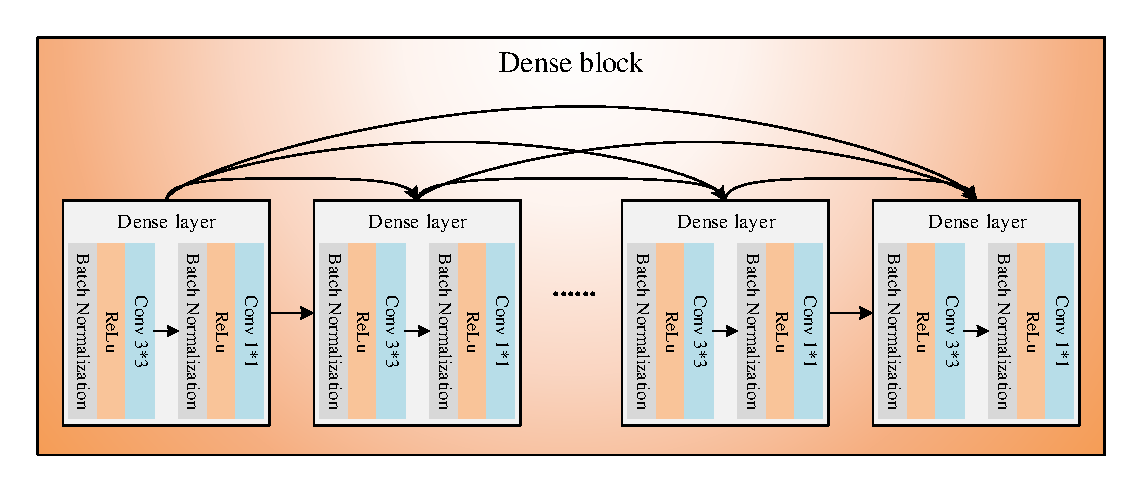
\includegraphics[
        width=0.78\textwidth,
        keepaspectratio
    ]{DenseBlock.pdf}
    \caption{The architecture of DenseNet.}
    \label{fig:DenseBlock}
\end{figure*} 

As for the DenseNet, different from a normal 
convolutional neural network, each dense 
layer’s output is fed to all subsequent dense 
layers in the same block through the dense 
connections, which is implemented by 
concatenation operations. In this way, global 
information can traverse the dense block from 
beginning to end, each dense layer can 
acquire extra knowledge from the previous ones. 
For a dense layer, it includes 2 basic layers, 
each basic layer is composed of a batch 
normalization layer, a ReLU activation 
function
\cite{Srivastava2014,Ioffe2015,Kingma2015} 
and 2 convolutional layers. The first 
convolutional layer with a 1 × 1 kernel is 
called the bottleneck layer, and it helps to 
reduce the feature map dimension to improve 
calculation efficiency. The second layer 
applies a 3 × 3 kernel to extract features. 
Benefit from densely connections, the network 
can extract more representative features than 
the normal convolutional network with layers 
connected in sequence. In addition, an 
attention block and a transition block are 
inserted between every two dense blocks. The 
attention block helps the feature extractors 
locate the most informative part of the 
input feature map. The transition block 
consists of a batch normalization layer 
and a 1 × 1 convolutional layer followed 
by 2 × 2 max pooling layer. It is set for 
down sampling the output feature maps of 
each dense block. While network goes deeper, 
the size of output feature maps decreases 
and the dimension of output feature maps 
increases. An example of the output feature 
maps after each dense block is shown in 
Figure~\ref{fig:imgFea}.

\begin{figure*}[!ht]
    \centering
    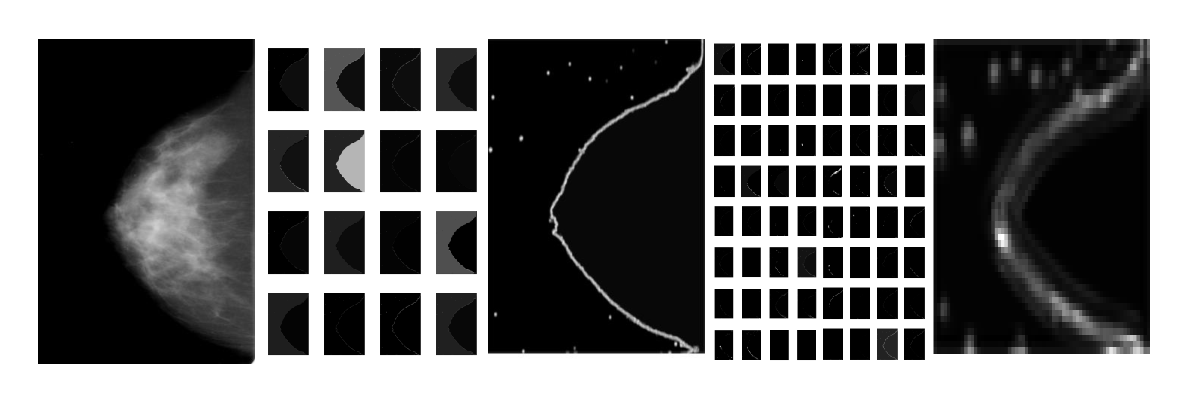
\includegraphics[
        width=1.0\textwidth,
        keepaspectratio
    ]{ImgFea.pdf}
    \caption{The feature of the 
        fusion of extractors' result.}
    \label{fig:imgFea}
\end{figure*} 

Usually, most CNN based methods on mammography 
image classification tasks use a single network 
to extract features, and then feed them into 
a classifier. However, we found that AGNet
did this job in a different way. It tried to 
explore the potential power of fusion features 
extracted from different models. In which, two 
models are fused to predict the label of input 
image together, one is based on AlexNet and  
there is based on GoogLeNet. It takes 
advantage of different features with higher 
accuracy than the single network methods.
Inspired by AGNet, proposing an approach to 
improve the classification accuracy by 
fusing multiple models with the same structure 
trained with different transfer learning 
strategies. Note that shallower layers tend to 
extract basic features, deeper layers tend to 
extract abstract feature, concluding that 
models with different layers’ parameters 
fixed during the training phase would focus on 
features with different complexity.
\cite{Ciresan2012}
At the inference phase, we fuse the trained models 
together to make use of the different 
feature extraction ability of each model.

Different from AGNet, train 3 models with 
the same structure, but freeze different 
layers of each model while training 
concurrently. There are two reasons why we 
select 3 same DenseNet based model to be fused. 
Firstly, we have tested the single-model 
method for this task, among which DenseNet
performs best. Secondly, we have tried fusing 
different trained models such as Inception, 
ResNet, DenseNet structures together with frozen 
parameters, fusing 3 DenseNet based models 
is still the better way. We think the reason 
is that when fusing models in different 
topological structures, the relationship 
between features extracted from 3 models is 
relatively weak and we cannot assure that 
they are learning different knowledge from 
training images. Since the structures of 
different networks varies greatly, models may
concentrate on similar features with different 
performance according to the depth of network. 
By training 4 similar structure models with 
different frozen layers, each model extracts 
features in different levels based on the 
number of frozen parameters, we can ensure 
that every model concentrates on different 
features of the input image. Meanwhile, in
the experiment we found the false positive 
and false negative instances of each model 
are quite different, which proves that they 
are concentrating on different kinds of 
features. Since the 4 models keep a similar 
network structure, the relationship between 
features they extracted are stronger,
and features can be fused better.

\begin{figure*}[!ht]
    \centering
    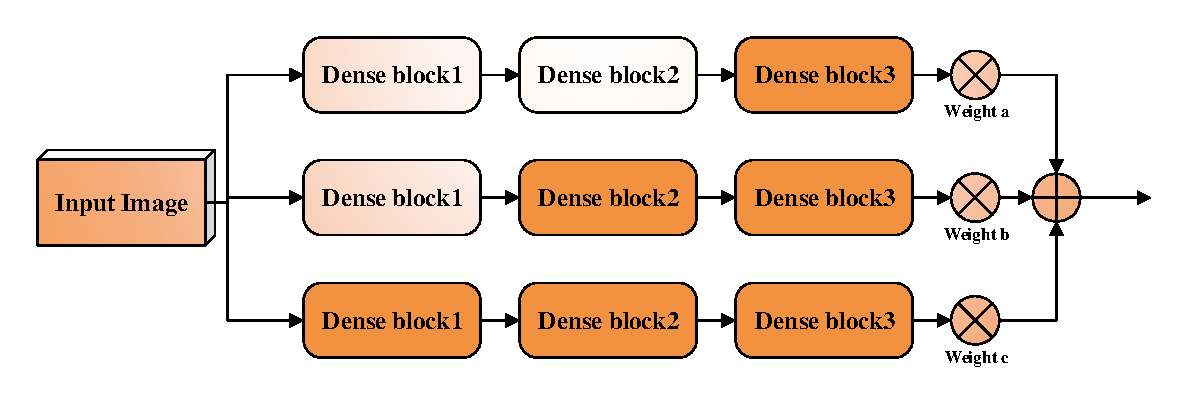
\includegraphics[
        width=0.78\textwidth,
        keepaspectratio
    ]{ExtractorFusion.pdf}
    \caption{The module of feature extractors' 
        fusion.}
    \label{fig:extrFusion}
\end{figure*} 

As figure~\ref{fig:extrFusion}
shows, training 3 models with parameters in 
different block frozen in parallel. Each row 
represents one model, the dense block in 
bright means that the parameters in this 
block are frozen during the training phase 
while the dark block means that parameters 
are activated. we fuse the feature of multiple 
transfer learning models with a weighted
sum operation. The weights of 3 models are 
set manually in the experiments. Taking the 
advantage of features diversity, the transfer 
learning models fusion method achieved high
accuracy in the mammography image recognition
task. 


\subsubsection{Hash Decoder Module}
\label{sec:MethNetHash}

After obtaining intermediate image features 
from the module of feature extractor, we
propose a hash decoder module to map these 
image features to hash codes. 
We assume each target hash code has q bits. 
Then the outputs of the feature extractor 
are designed to be 50q. As can be seen in 
Figure~\ref{fig:hashDecoder}, 
the proposed hash decoder module firstly 
divides randomly the features vectors into 
q slices with equal length 4. Then each 
slice is mapped to one dimension by a 
fully-connected layer, followed by a 
sigmoid activation function that restricts 
the output value in the range [0, 1],
and a piece-wise threshold function to 
encourage the output of binary hash bits. 
After that, the q output hash bits are
concatenated to be a q-bit code. A possible 
alternative to the hash decoder module is 
a simple fully-connected layer that maps 
the input intermediate image features into 
q-dimensional vectors, followed by sigmoid 
activation functions to transform these 
vectors into [0, 1]. Compared to this 
alternative, the key idea of the overall 
strategy is trying to reduce the redundancy 
among the hash bits. Hash codes with fewer 
redundant bits are advocated by some recent 
research. 

\begin{figure*}[!ht]
    \centering
    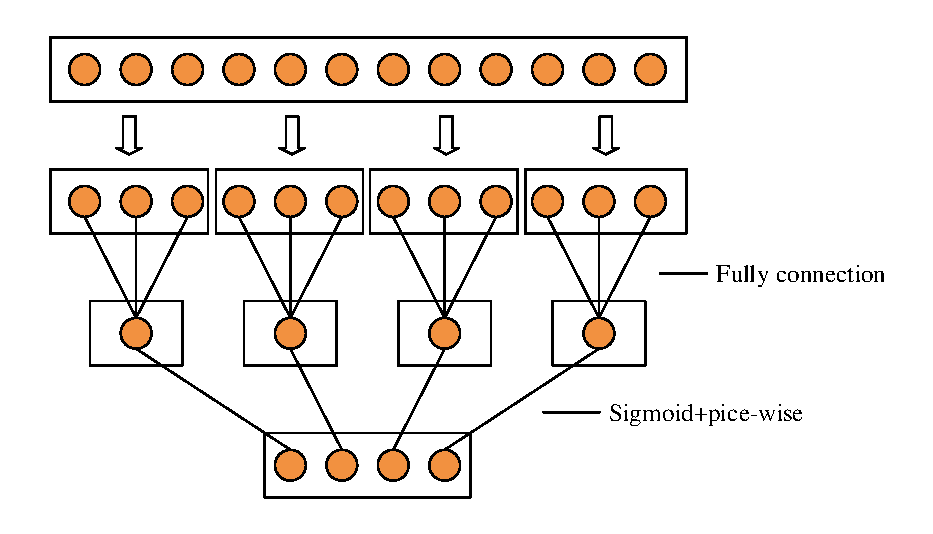
\includegraphics[
        width=0.66\textwidth,
        keepaspectratio
    ]{HashDecode.pdf}
    \caption{The module of the hash decoder.}
    \label{fig:hashDecoder}
\end{figure*} 

In order to encourage the output of a hash 
decoder to be binary codes, we use a sigmoid 
activation function followed by a piece-wise 
threshold function.
Given a 50-dimensional slice 
$x^{(i)}(i=1,2,...q)$
, the output of the 50-to-1 fully-connected 
layer is defined by

\begin{equation}
    \label{eq:eq_descr_1}
    fc_i(x^{(i)}) = W_ix^{(i)}
\end{equation}

with $W_i$ being the weight matrix.

Given $c=fc_i(x^{(i)})$, the sigmoid function
is defined by 

\begin{equation}
    \label{eq:eq_descr_2}
    sigmoid(c) = \frac{1}{1+e^{-\beta c}}
\end{equation}

where $\beta$ is a hyper-parameter.

The piece-wise threshold function is to 
encourage binary outputs. Specifically, for an 
input variable $s = sigmoid(c) \in [0,1]$, 
this piece-wise function is defined by

\begin{equation}
    \label{eq:eq_descr_3}
    y = \left\{
        \begin{array}{lr}
            0, & s < 0.5-\epsilon \\
            s, & 0.5-\epsilon \le 0.5+\epsilon \\
            1, & s > 0.5+\epsilon
        \end{array}
    \right.\nonumber,
\end{equation}

where $\epsilon$ is a small positive 
hyper-parameter.

This piece-wise threshold function 
approximates the behavior of hard-coding, 
and it encourages binary outputs in training. 
Specifically, if the outputs from the sigmoid 
function are in $[0, 0.5-\epsilon]$ or 
$[0.5+\epsilon, 1]$, they are truncated to be 
0 or 1, respectively. Note that in prediction, 
the proposed deep architecture only generates 
approximate (real-value) hash codes for input 
images, where these approximate codes are 
converted to binary codes by quantization. 
With the proposed piece-wise threshold 
function, some of the values in the 
approximate hash codes are already zeros or 
ones. Hence, less errors may be introduced
by the quantization step.

\subsubsection{Classifier Module}
\label{sec:MethNetCls}

In the classifier module, building it with
a fusion structure by SVM, KNN, Random
Forest classic methods. For each method, it 
predicates with the output of the hash decoder,
then the three results weight add, as the 
result of class information. There is a reason
why we select 3 different classifiers to be 
fused. These three algorithms target 
different classification types, so the 
results obtained for different feature 
information will also be different. The 
biggest advantage of doing this is to 
improve the robustness of the model, 
and at the same time it also improves 
the accuracy of model recognition. 

\begin{figure*}[!ht]
    \centering
    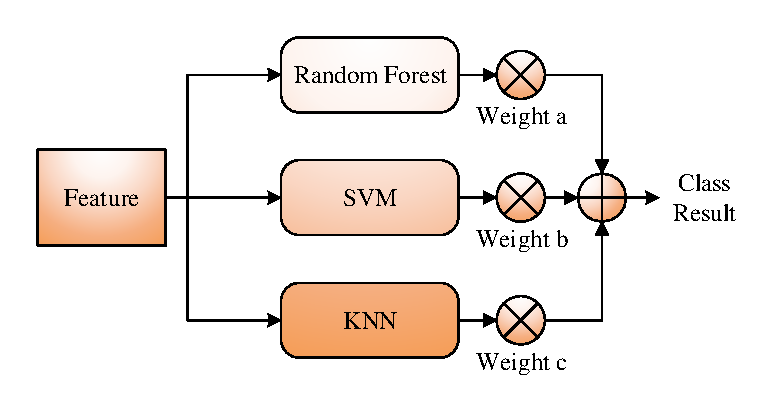
\includegraphics[
        width=0.58\textwidth,
        keepaspectratio
    ]{ClassifierFusion.pdf}
    \caption{The module of the fusion of 
        classifier.}
    \label{fig:classifierFusion}
\end{figure*}   

As for the KNN, which is simple, easy to 
understand, easy to implement, no need 
to estimate parameters, no training. 
As for the SVM,  after the training is 
completed, most of the training samples 
do not need to be retained, and the final 
model is only related to the support vector.
As for the Random Forest, which is based on 
an ensemble of decision trees where each of the 
trees is based on the randomly selected subset of 
the training set. Random forest uses slightly 
different kinds of bagging approach where a 
subset of features is selected for the split
at node, whereas in bagging all features are 
used for node split. As a result, the random 
forest is an aggregation of trees, which reduces 
the effect of noise present in a single tree.
Hence, bagging generally increases the 
overall result.

\subsubsection{Regression module}
\label{sec:MethNetReg}

A Region Proposal Network (RPN) takes an 
image (of any size) as input and outputs a 
set of rectangular object proposals, 
each with an objectness score. To generate 
region proposals, sliding a small network 
over the conv feature map output by the last
shared conv layer. This network is 
fully connected to an n × n spatial window 
of the input conv feature map. Each sliding 
window is mapped to a lower-dimensional vector. 
This vector is fed into two sibling 
fully-connected layers — a box-regression layer 
and a box-classification layer. As shown in
Figure~\ref{fig:RPN}

\begin{figure*}[!ht]
    \centering
    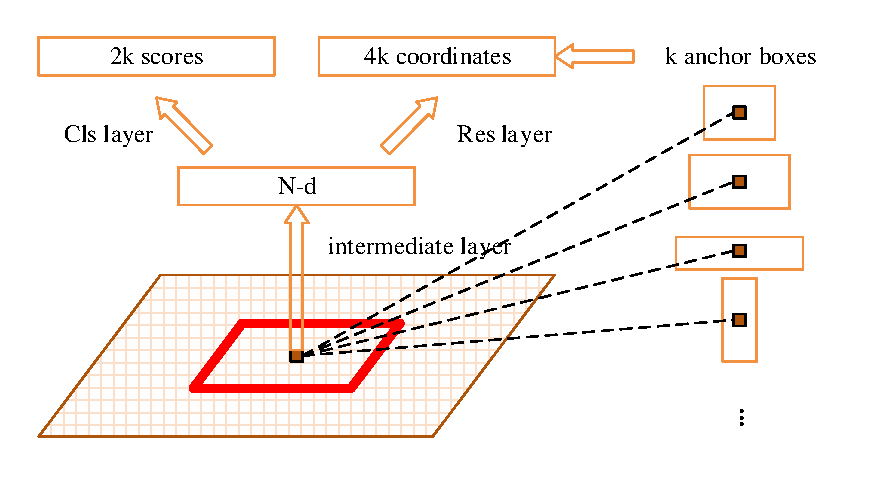
\includegraphics[
        width=0.68\textwidth,
        keepaspectratio
    ]{RPN.pdf}
    \caption{The module of the region proposal 
        network.}
    \label{fig:RPN}
\end{figure*} 


Note that because the mini-network operates
in a sliding-window fashion, the 
fully-connected layers are shared across 
all spatial locations. This architecture is 
naturally implemented with an n × n conv layer 
followed by two sibling 1 × 1 conv
layers. And the loss function is defined by

\begin{equation}
    \label{eq:eq_descr_4}
    L({p_i},{t_i})=\frac{1}{N_{cls}}\sum_iL_{cls}(p_i,p_i^*)
     + \lambda\frac{1}{N_{reg}}\sum_ip_i^*L_{reg}(t_i,t_i^*)
\end{equation}

Here, $i$ is the index of an anchor in a 
mini-batch and $p_i$ is the predicted 
probability of anchor $i$ being an object. 
The ground-truth label $p_i^*$ is 1 if the 
anchor is positive, and is 0 if the anchor 
is negative. $t_i$ is a vector representing 
the 4 parameterized coordinates of the 
predicted bounding box, and $t_i^*$ is that
of the ground-truth box associated with a 
positive anchor. The classification loss 
$L_{cls}$ is log loss over two classes 
(object $vs$ not object). For the regression 
loss, we use 
$L_{reg}(t_i, t_i^*)=R(t_i, t_i^*)$ where $R$
is the robust loss function (smooth $L_i$). 
The term $p_i^*L_{reg}$ means the regression 
loss is activated only for positive anchors 
and is disabled otherwise. The outputs of
the $cls$ and $reg$ layers consist of ${p_i}$ 
and ${t_i}$ respectively. The two terms are 
normalized with $N_{cls}$ and $N_{reg}$, and 
a balancing weight $\lambda$.

For regression, we adopt the parameterizations 
of the 4 coordinates following:

\begin{eqnarray}\label{eq:eq_descr_5}
    t_x=(x-x_a)/w_a, 
    t_y=(y-y_a)/h_a, 
    t_w=log(w/w_a), 
    t_h=log(h/h_a), \\
    t_x^*=(x^*-x^*_a)/w_a, 
    t_y^*=(y^*-y^*_a)/h_a, 
    t_w^*=log(w^*/w_a), 
    t_h^*=log(h^*/h_a)
\end{eqnarray}

where $x$, $y$, $w$, and $h$ denote the two 
coordinates of the box center, width, and 
height. Variables $x$, $x_a$, and $x^*$ are 
for the predicted box, anchor box, and 
ground-truth box respectively (likewise for 
$y$, $w$, $h$). This can be thought of as 
bounding-box regression from an anchor box 
to a nearby ground-truth box.

\subsection{Transfer learning}
\label{sec:MethTL}

Transfer learning aims to transfer knowledge 
between related source and target domains
\cite{Pan2010}.
It is a useful tool in machine learning, 
leading to a positive effect on the domains 
that are difficult to apply because of 
insufficient training data. Transfer learning 
methods can be categorized into 4 classes: 
instance-based, mapping-based, network-based,
adversarial-based deep transfer learning
\cite{Tan2018}.
Network-based method is mostly used in 
convolutional neural networks. It is achieved 
by transferring the network structure and 
pre-trained parameters of the source domain into 
a part of a deep convolutional neural network 
used in the target domain. In our work, 
we construct feature extractor as 
described in Section~\ref{sec:MethNetFea}, 
then we initialize the network parameters 
with the parameters of a DenseNet model 
that were pre-trained on the ImageNet dataset.

In our experiments, an input image is 
resized to a tensor, going that dataset; 
freezing, which consists of leaving the 
parameters in shallow part of the 
pretrained model unchanged and training 
only the rest part of the network, which can 
make use of the basic feature extracting 
ability of pretrained model. Freezing layers 
or not in training phase depends on the 
number of category and quantity variance 
between source and target dataset. 
Compared to ImageNet dataset, the DDSM 
dataset we used are much smaller. 
Moreover, most images in both datasets 
are natural images, they are similar in 
a way, hence we freeze some of the layers 
during training. In order to explore the 
effect of fusing different feature extractors, 
we try different freezing strategy on the 
networks, the details are described in 
Section~\ref{sec:MethNetFea}. 
